\documentclass[12pt,letterpaper]{article}
\usepackage{graphicx,textcomp}
\usepackage{natbib}
\usepackage{setspace}
\usepackage{fullpage}
\usepackage{color}
\usepackage[reqno]{amsmath}
\usepackage{amsthm}
\usepackage{fancyvrb}
\usepackage{amssymb,enumerate}
\usepackage[all]{xy}
\usepackage{endnotes}
\usepackage{lscape}
\newtheorem{com}{Comment}
\usepackage{float}
\usepackage{hyperref}
\newtheorem{lem} {Lemma}
\newtheorem{prop}{Proposition}
\newtheorem{thm}{Theorem}
\newtheorem{defn}{Definition}
\newtheorem{cor}{Corollary}
\newtheorem{obs}{Observation}
\usepackage[compact]{titlesec}
\usepackage{dcolumn}
\usepackage{tikz}
\usetikzlibrary{arrows}
\usepackage{multirow}
\usepackage{xcolor}
\newcolumntype{.}{D{.}{.}{-1}}
\newcolumntype{d}[1]{D{.}{.}{#1}}
\definecolor{light-gray}{gray}{0.65}
\usepackage{url}
\usepackage{listings}
\usepackage{color}

\definecolor{codegreen}{rgb}{0,0.6,0}
\definecolor{codegray}{rgb}{0.5,0.5,0.5}
\definecolor{codepurple}{rgb}{0.58,0,0.82}
\definecolor{backcolour}{rgb}{0.95,0.95,0.92}

\lstdefinestyle{mystyle}{
	backgroundcolor=\color{backcolour},   
	commentstyle=\color{codegreen},
	keywordstyle=\color{magenta},
	numberstyle=\tiny\color{codegray},
	stringstyle=\color{codepurple},
	basicstyle=\footnotesize,
	breakatwhitespace=false,         
	breaklines=true,                 
	captionpos=b,                    
	keepspaces=true,                 
	numbers=left,                    
	numbersep=5pt,                  
	showspaces=false,                
	showstringspaces=false,
	showtabs=false,                  
	tabsize=2
}
\lstset{style=mystyle}
\newcommand{\Sref}[1]{Section~\ref{#1}}
\newtheorem{hyp}{Hypothesis}

\title{Problem Set 1}
\date{Due: October 1, 2021}
\author{Applied Stats/Quant Methods 1}

\begin{document}
	\maketitle
	
	\section*{Instructions}
	\begin{itemize}
		\item Please show your work! You may lose points by simply writing in the answer. If the problem requires you to execute commands in \texttt{R}, please include the code you used to get your answers. Please also include the \texttt{.R} file that contains your code. If you are not sure if work needs to be shown for a particular problem, please ask.
		\item Your homework should be submitted electronically on GitHub in \texttt{.pdf} form.
		\item This problem set is due before 8:00 on Friday October 1, 2021. No late assignments will be accepted.
		\item Total available points for this homework is 100.
	\end{itemize}
	
	\vspace{1cm}
	\section*{Question 1 (50 points): Education}

A school counselor was curious about the average of IQ of the students in her school and took a random sample of 25 students' IQ scores. The following is the data set:\\
\vspace{.5cm}

\lstinputlisting[language=R, firstline=40, lastline=40]{PS01.R}  

\vspace{1cm}

\begin{enumerate}
	\item Find a 90\% confidence interval for the average student IQ in the school.\\
	
	\item Next, the school counselor was curious  whether  the average student IQ in her school is higher than the average IQ score (100) among all the schools in the country.\\ 
	
	\noindent Using the same sample, conduct the appropriate hypothesis test with $\alpha=0.05$.
\end{enumerate}

\vspace{1cm}
\section*{Answer 1}

\begin{enumerate}
	\item I first loaded the variable y which was already provided. To estimate the confidence interval of 90\% I transformed it into .10 coefficient used in the following formula:
\lstinputlisting[language=R, firstline=44, lastline=44]{PS01_AC_Answer.R} 
	This formula provided me with the value of Z score is 1.644. Further, I estimated the number of cases (25) and calculated the sample mean (98.44) and standard deviation (13.09) using available R functions:
\lstinputlisting[language=R, firstline=45, lastline=47]{PS01_AC_Answer.R}	
	Even though na.rm function is not necessary in this case, I left it because it does not create any problems in the calculation. I then proceeded with a standard formula for calculating the confidence interval. I used two tailed confidence intervals and calculated both upper and lower tail: 
\lstinputlisting[language=R, firstline=48, lastline=50]{PS01_AC_Answer.R}
	Using this formula for variable y, I estimated that the confidence interval lies between 94.1 and 102.7.	
	
	\item To check if the average student IQ in the school is the same as average student IQ in the country (= 100) I used a t.test function in R. Before calculating the t test I set up null and alternative hypothesis. Having in mind I already had the sample mean from the previous task, I assumed that the mean of the students in school is not the same as the mean in the country (98.44:100). Therefore my null and alternative hypotheses were defined as following:
	\begin{enumerate}
		\item H0: Sample mean = Country mean;
		\item Ha: Sample mean =/= Country mean;
	\end{enumerate} 
I then tested my hypothesis using the following t test features:
	\lstinputlisting[language=R, firstline=61, lastline=62]{PS01_AC_Answer.R}
As per R help guidelines and the tutorial script I did this one-sample t test using y as my sample; mu took the value of 100 as a expected true value of the mean and as per task I took the confidence interval of .05. The results of my t test are the following: t = -0.59574, df = 24, p-value = 0.5569. The 5\% confidence interval lies between 98.27407 and 98.60593 while mean is 98.44 (same as in the previous task). As per R output, the alternative hypothesis that sample mean and country mean are not the same is corroborated. Yet the value of p (0.5569) is bigger than the confidence level of .05 which tells that the null hypothesis cannot be rejected.  
\end{enumerate}


\newpage

	\section*{Question 2 (50 points): Political Economy}

\noindent Researchers are curious about what affects the amount of money communities spend on addressing homelessness. The following variables constitute our data set about social welfare expenditures in the USA. \\
\vspace{.5cm}


\begin{tabular}{r|l}
	\texttt{State} &\emph{50 states in US} \\
	\texttt{Y} & \emph{per capita expenditure on shelters/housing assistance in state}\\
	\texttt{X1} &\emph{per capita personal income in state} \\
	\texttt{X2} &  \emph{Number of residents per 100,000 that are "financially insecure" in state}\\
	\texttt{X3} &  \emph{Number of people per thousand residing in urban areas in state} \\
	\texttt{Region} &  \emph{1=Northeast, 2= North Central, 3= South, 4=West} \\
\end{tabular}

\vspace{.5cm}
\noindent Explore the \texttt{expenditure} data set and import data into \texttt{R}.
\vspace{.5cm}
\lstinputlisting[language=R, firstline=54, lastline=54]{PS01.R}  
\vspace{.5cm}
\begin{itemize}

\item
Please plot the relationships among \emph{Y}, \emph{X1}, \emph{X2}, and \emph{X3}? What are the correlations among them (you just need to describe the graph and the relationships among them)?
\vspace{.5cm}
\item
Please plot the relationship between \emph{Y} and \emph{Region}? On average, which region has the highest per capita expenditure on housing assistance?
\vspace{.5cm}
\item
Please plot the relationship between \emph{Y} and \emph{X1}? Describe this graph and the relationship. Reproduce the above graph including one more variable \emph{Region} and display different regions with different types of symbols and colors.
\end{itemize}

\section*{Answer 2}

\begin{enumerate}
	\item As part of the Q2 1st task I loaded the expenditure table. I inspected the following data frame using the following functions:
	\lstinputlisting[language=R, firstline=71, lastline=76]{PS01_AC_Answer.R}
	I ran all of them to test the features of R and repeat ways of inspecting variables and datasets from the coding camp and the tutorial. 
	
	Doing the first task I was not sure how to get the best graphics with barplot function in R, so I loaded ggplot2:
	\lstinputlisting[language=R, firstline=25, lastline=25]{PS01_AC_Answer.R}
	I used option qplot to render graphics of variable y (per capita expenditure on shelters/housing assistance in state) with X1 (per capita personal income in state), X2 (Number of residents per 100,000 that are "financially insecure" in state) and X3 (Number of people per thousand residing in urban areas in state) separately: 
	\lstinputlisting[language=R, firstline=79, lastline=81]{PS01_AC_Answer.R}
	Using qplot, I rendered the following graphs:
	
	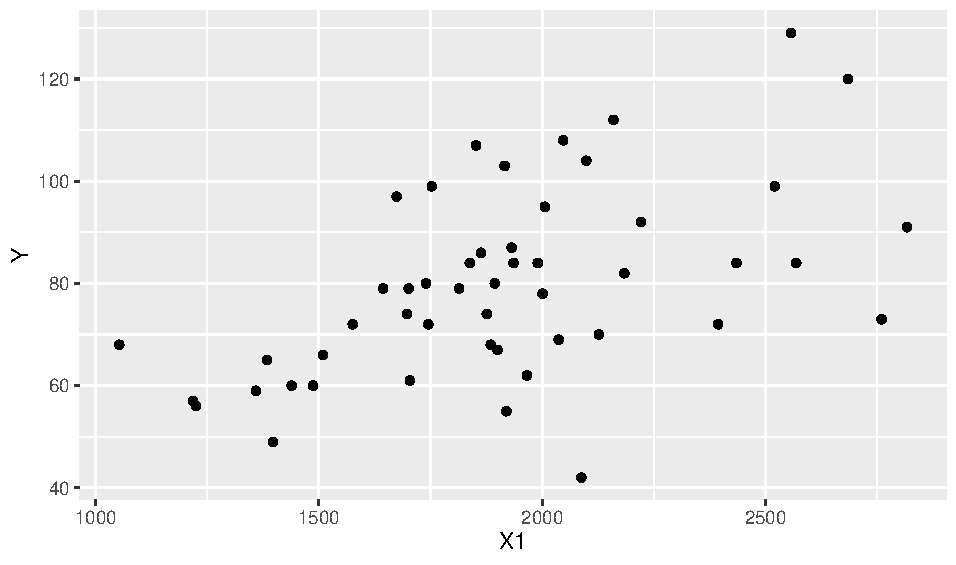
\includegraphics{Qplot11}
	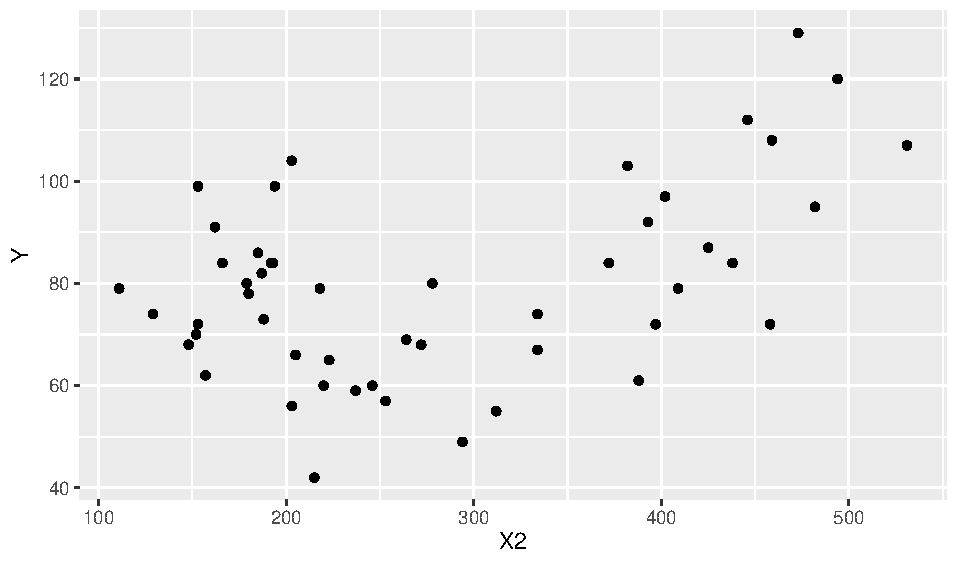
\includegraphics{Qplot21}
	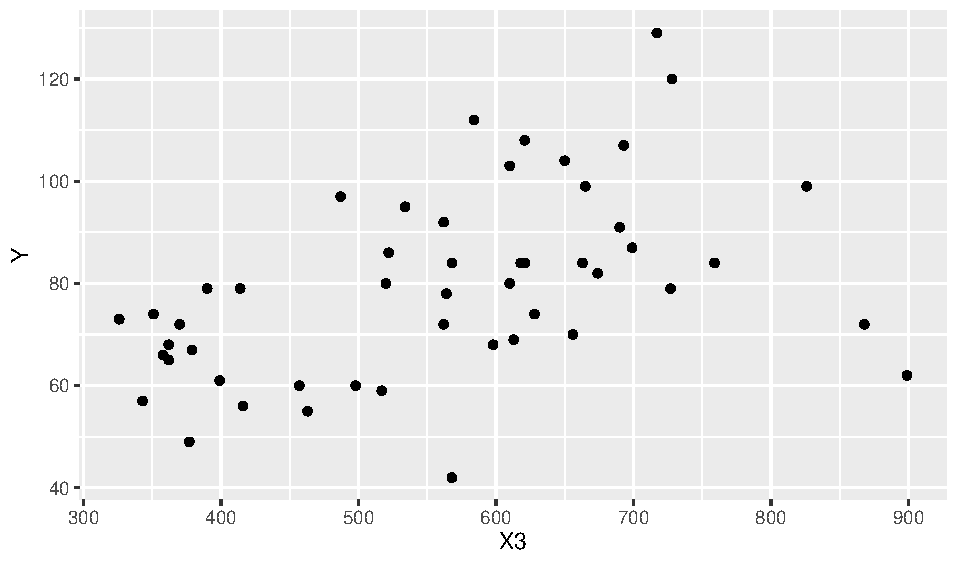
\includegraphics{Qplot3}
	
	On each graph I put Y (per capita expenditure on shelters/housing assistance in state) on the y axis, while the X1, X2 and X3 were put on the X axis. In the first plot there seem to be a slight correlation between Y and X1 (per capita personal income in state). This correlation seem to exist until the income reaches a point of 1750\$ after which the data become more disperse. On the second graph, the relationship per capita expenditure on shelters/housing assistance in state and the number of residents per 100,000 that are "financially insecure" in state does not show a visible trend due to dispersed data until the number of financially insecure residents reaches 300 after which the increasing trend becomes visible. On the third graph, that depicts the relationship between per capita expenditure on shelters/housing assistance in state and a number of people per thousand residing in urban areas in state no clear trend could be observed due to highly dispersed data. 
	
	\item To plot the relationship between Y and Region (1=Northeast, 2= North Central, 3= South, 4=West) I used barplot function in R. In the first line I aggregated the data for per capita expenditure on shelters/housing assistance and listed them per regions:   
	 
	\lstinputlisting[language=R, firstline=84, lastline=91]{PS01_AC_Answer.R}
	
	This code rendered the following bar chart:
	
	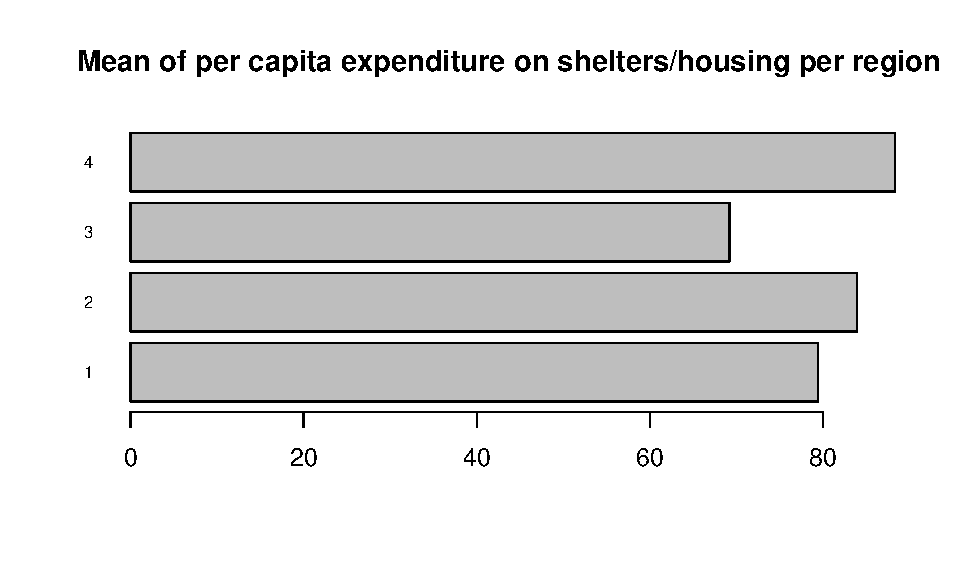
\includegraphics{Barplot}
	
	From this graph it is visible that the highest amount of per capita expenses is in the 4th region (West), while the lowest level is in the 3rd region (South).  
	
	\item To resolve the third task, I used ggplot2 again. Inside ggplot I used colour option to indicate the differences among regions while plotting the relationship between per capita expenditure and per capita personal income. Before rendering the graph I created and new variable Region1, overwriting Region as factor variable: 
	
	\lstinputlisting[language=R, firstline=95, lastline=95]{PS01_AC_Answer.R}  
	
	I put per capita expenditure on y axis and per capita personal income in state on x axis (in accordance with previous graphs). The code rendered the following graph:
	
	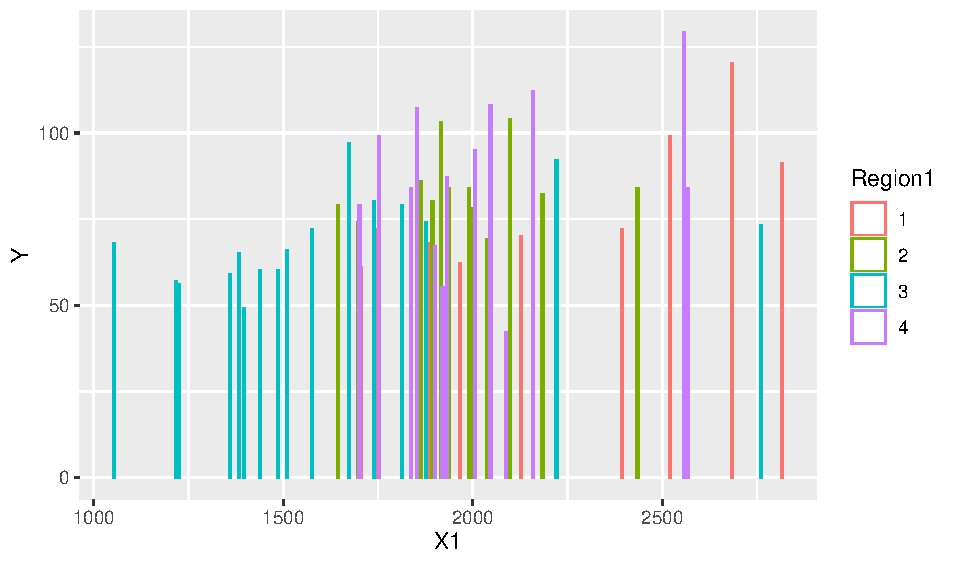
\includegraphics{Ggplot}
	
	From this graph it is visible that the lowest level of per capita income correlates the lowest levels of expenditure which are most common in the southern states. On average the highest amount of expenditure is most densely concentrated in the region around \$2000 income level.    
	
	   
	
	
\end{enumerate}

\end{document}
